\documentclass[tikz,convert]{standalone}

\usetikzlibrary{decorations.pathreplacing}
\usetikzlibrary{snakes}

\begin{document}
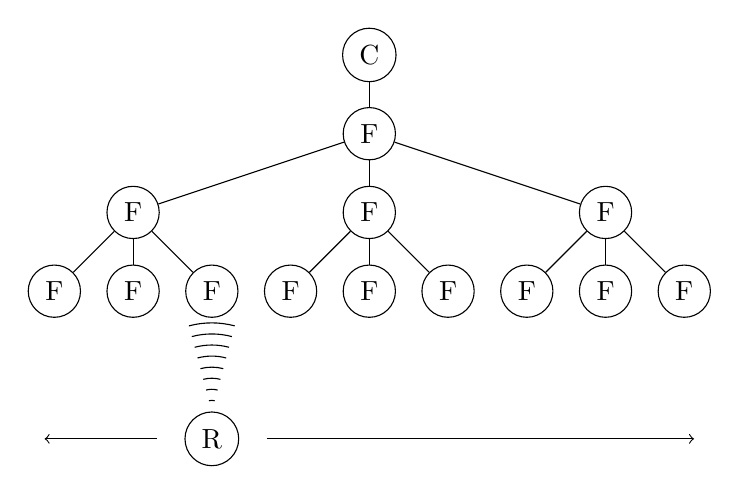
\begin{tikzpicture}

  % Network edge nodes
  \node[draw, shape=circle] (e11) {F};
  \node[draw, shape=circle, right of=e11] (e12) {F};
  \node[draw, shape=circle, right of=e12] (e13) {F};
  \node[draw, shape=circle, right of=e13] (e21) {F};
  \node[draw, shape=circle, right of=e21] (e22) {F};
  \node[draw, shape=circle, right of=e22] (e23) {F};
  \node[draw, shape=circle, right of=e23] (e31) {F};
  \node[draw, shape=circle, right of=e31] (e32) {F};
  \node[draw, shape=circle, right of=e32] (e33) {F};
  % Network core nodes
  \node[draw, shape=circle, above of=e12] (c10) {F};
  \node[draw, shape=circle, above of=e22] (c20) {F};
  \node[draw, shape=circle, above of=e32] (c30) {F};
  \node[draw, shape=circle, above of=c20] (c00) {F};
  \node[draw, shape=circle, above of=c00] (c) {C};
  % Moving repo
  \node[draw, shape=circle, below of=e13, below=15pt] (r) {R};

  % Network core connections
  \path[draw,-] (c) to (c00);
  \path[draw,-] (c00) to (c10);
  \path[draw,-] (c00) to (c20);
  \path[draw,-] (c00) to (c30);
  % Network edge connections
  \path[draw,-] (c10) to (e11);
  \path[draw,-] (c10) to (e12);
  \path[draw,-] (c10) to (e13);
  \path[draw,-] (c20) to (e21);
  \path[draw,-] (c20) to (e22);
  \path[draw,-] (c20) to (e23);
  \path[draw,-] (c30) to (e31);
  \path[draw,-] (c30) to (e32);
  \path[draw,-] (c30) to (e33);

  % Hidden nodes for repo moving anchors
  \path[draw=none] (e11) |- (r) node[pos=.5] (rl) {};
  \path[draw=none] (e33) |- (r) node[pos=.5] (rr) {};
  % Repo moving arrows
  \path[draw,->] (r.west) ++ (-10pt, 0) to (rl.west);
  \path[draw,->] (r.east) ++ (10pt, 0) to (rr.east);

  % Radio waves between repo and e13
  \path[draw, snake=expanding waves, segment length=4pt, segment angle=15] (r.north) to (e13.south);
  
\end{tikzpicture}
\end{document}
